% Options for packages loaded elsewhere
\PassOptionsToPackage{unicode}{hyperref}
\PassOptionsToPackage{hyphens}{url}
\PassOptionsToPackage{dvipsnames,svgnames,x11names}{xcolor}
\documentclass[
  american,
  11pt,
  a4paper,
]{article}
\usepackage{xcolor}
\usepackage{microtype}
\usepackage[margin=1in]{geometry}
\usepackage{amsmath,amssymb}
\setcounter{secnumdepth}{-\maxdimen} % remove section numbering
\usepackage{iftex}
\ifPDFTeX
  \usepackage[T1]{fontenc}
  \usepackage[utf8]{inputenc}
  \usepackage{textcomp} % provide euro and other symbols
\else % if luatex or xetex
  \usepackage{unicode-math} % this also loads fontspec
  \defaultfontfeatures{Scale=MatchLowercase}
  \defaultfontfeatures[\rmfamily]{Ligatures=TeX,Scale=1}
\setmonofont{Cascadia Mono}
\fi
\usepackage{lmodern}
\ifPDFTeX\else\setmonofont{Cascadia Mono}\fi
\ifPDFTeX\else
  % xetex/luatex font selection
\fi
% Use upquote if available, for straight quotes in verbatim environments
\IfFileExists{upquote.sty}{\usepackage{upquote}}{}
\IfFileExists{microtype.sty}{% use microtype if available
  \usepackage[]{microtype}
  \UseMicrotypeSet[protrusion]{basicmath} % disable protrusion for tt fonts
}{}
\makeatletter
\@ifundefined{KOMAClassName}{% if non-KOMA class
  \IfFileExists{parskip.sty}{%
    \usepackage{parskip}
  }{% else
    \setlength{\parindent}{0pt}
    \setlength{\parskip}{6pt plus 2pt minus 1pt}}
}{% if KOMA class
  \KOMAoptions{parskip=half}}
\makeatother
\usepackage{color}
\usepackage{fancyvrb}
\usepackage{fvextra}
\usepackage[htt]{hyphenat}
\newcommand{\VerbBar}{|}
\newcommand{\VERB}{\Verb[commandchars=\\\{\}]}
\DefineVerbatimEnvironment{Highlighting}{Verbatim}{commandchars=\\\{\},breaklines=true,breakanywhere=true,fontsize=\small}
% Add ',fontsize=\small' for more characters per line
\newenvironment{Shaded}{}{}
\newcommand{\AlertTok}[1]{\textcolor[rgb]{1.00,0.00,0.00}{\textbf{#1}}}
\newcommand{\AnnotationTok}[1]{\textcolor[rgb]{0.38,0.63,0.69}{\textbf{\textit{#1}}}}
\newcommand{\AttributeTok}[1]{\textcolor[rgb]{0.49,0.56,0.16}{#1}}
\newcommand{\BaseNTok}[1]{\textcolor[rgb]{0.25,0.63,0.44}{#1}}
\newcommand{\BuiltInTok}[1]{\textcolor[rgb]{0.00,0.50,0.00}{#1}}
\newcommand{\CharTok}[1]{\textcolor[rgb]{0.25,0.44,0.63}{#1}}
\newcommand{\CommentTok}[1]{\textcolor[rgb]{0.38,0.63,0.69}{\textit{#1}}}
\newcommand{\CommentVarTok}[1]{\textcolor[rgb]{0.38,0.63,0.69}{\textbf{\textit{#1}}}}
\newcommand{\ConstantTok}[1]{\textcolor[rgb]{0.53,0.00,0.00}{#1}}
\newcommand{\ControlFlowTok}[1]{\textcolor[rgb]{0.00,0.44,0.13}{\textbf{#1}}}
\newcommand{\DataTypeTok}[1]{\textcolor[rgb]{0.56,0.13,0.00}{#1}}
\newcommand{\DecValTok}[1]{\textcolor[rgb]{0.25,0.63,0.44}{#1}}
\newcommand{\DocumentationTok}[1]{\textcolor[rgb]{0.73,0.13,0.13}{\textit{#1}}}
\newcommand{\ErrorTok}[1]{\textcolor[rgb]{1.00,0.00,0.00}{\textbf{#1}}}
\newcommand{\ExtensionTok}[1]{#1}
\newcommand{\FloatTok}[1]{\textcolor[rgb]{0.25,0.63,0.44}{#1}}
\newcommand{\FunctionTok}[1]{\textcolor[rgb]{0.02,0.16,0.49}{#1}}
\newcommand{\ImportTok}[1]{\textcolor[rgb]{0.00,0.50,0.00}{\textbf{#1}}}
\newcommand{\InformationTok}[1]{\textcolor[rgb]{0.38,0.63,0.69}{\textbf{\textit{#1}}}}
\newcommand{\KeywordTok}[1]{\textcolor[rgb]{0.00,0.44,0.13}{\textbf{#1}}}
\newcommand{\NormalTok}[1]{#1}
\newcommand{\OperatorTok}[1]{\textcolor[rgb]{0.40,0.40,0.40}{#1}}
\newcommand{\OtherTok}[1]{\textcolor[rgb]{0.00,0.44,0.13}{#1}}
\newcommand{\PreprocessorTok}[1]{\textcolor[rgb]{0.74,0.48,0.00}{#1}}
\newcommand{\RegionMarkerTok}[1]{#1}
\newcommand{\SpecialCharTok}[1]{\textcolor[rgb]{0.25,0.44,0.63}{#1}}
\newcommand{\SpecialStringTok}[1]{\textcolor[rgb]{0.73,0.40,0.53}{#1}}
\newcommand{\StringTok}[1]{\textcolor[rgb]{0.25,0.44,0.63}{#1}}
\newcommand{\VariableTok}[1]{\textcolor[rgb]{0.10,0.09,0.49}{#1}}
\newcommand{\VerbatimStringTok}[1]{\textcolor[rgb]{0.25,0.44,0.63}{#1}}
\newcommand{\WarningTok}[1]{\textcolor[rgb]{0.38,0.63,0.69}{\textbf{\textit{#1}}}}
\usepackage{longtable,booktabs,array}
\newcounter{none} % for unnumbered tables
\usepackage{calc} % for calculating minipage widths
% Correct order of tables after \paragraph or \subparagraph
\usepackage{etoolbox}
\makeatletter
\patchcmd\longtable{\par}{\if@noskipsec\mbox{}\fi\par}{}{}
\makeatother
% Allow footnotes in longtable head/foot
\IfFileExists{footnotehyper.sty}{\usepackage{footnotehyper}}{\usepackage{footnote}}
\makesavenoteenv{longtable}
\usepackage{graphicx}
\makeatletter
\newsavebox\pandoc@box
\newcommand*\pandocbounded[1]{% scales image to fit in text height/width
  \sbox\pandoc@box{#1}%
  \Gscale@div\@tempa{\textheight}{\dimexpr\ht\pandoc@box+\dp\pandoc@box\relax}%
  \Gscale@div\@tempb{\linewidth}{\wd\pandoc@box}%
  \ifdim\@tempb\p@<\@tempa\p@\let\@tempa\@tempb\fi% select the smaller of both
  \ifdim\@tempa\p@<\p@\scalebox{\@tempa}{\usebox\pandoc@box}%
  \else\usebox{\pandoc@box}%
  \fi%
}
% Set default figure placement to htbp
\def\fps@figure{htbp}
\makeatother
\ifLuaTeX
\usepackage[bidi=basic,shorthands=off]{babel}
\else
\usepackage[bidi=default,shorthands=off]{babel}
\fi
\ifLuaTeX
  \usepackage{selnolig} % disable illegal ligatures
\fi
\setlength{\emergencystretch}{8em} % prevent overfull lines
\providecommand{\tightlist}{%
  \setlength{\itemsep}{0pt}\setlength{\parskip}{0pt}}
\usepackage{bookmark}
\IfFileExists{xurl.sty}{\usepackage{xurl}}{} % add URL line breaks if available
\urlstyle{same}
\hypersetup{
  pdftitle={Affine Profile Reduction for Fractional Triangle Packings in Split Graphs},
  pdfauthor={AUTHORBLOCK},
  pdflang={en-US},
  colorlinks=true,
  linkcolor={blue},
  filecolor={Maroon},
  citecolor={Blue},
  urlcolor={blue},
  pdfcreator={LaTeX via pandoc}}

\title{Affine Profile Reduction for Fractional Triangle Packings in Split Graphs}
\author{Juan Pablo Traverso Gianini\\
\small Independent researcher, Santiago, Chile\\
\small \href{mailto:jtraverso@gmail.com}{jtraverso@gmail.com}\\
\small ORCID: 0009-0003-6068-4096}
\date{}

% Series layout authority: official GitHub preprint template (article, 11pt, A4, 1in).
% Generated from the language-specific Markdown semantic source.
\AtBeginEnvironment{longtable}{\scriptsize}
\begin{document}
\sloppy
\raggedbottom
\maketitle

\textbf{Paper I in the series}\\
\textbf{Preprint:} version 1.3. This manuscript and its accompanying formal artifact form one self-contained public package.\\
\textbf{Release date:} August 22, 2026\\
\textbf{Status:} official author preprint release. The accompanying Paper I Lean v1.2 freeze includes the recorded build evidence and theorem-level axiom queries described in Section 10. The exact archive and manuscript package passed independent external adversarial review. This release is not external human peer review or a specialist priority determination.

\textbf{Prior-art and novelty status.} The internal literature audit, supplemented by external adversarial review, identified no earlier result with the same finite fractional split-graph bound and affine-profile reduction. The broader chordal clique-partition problem remains open. This is a corpus-bounded negative search, not proof of priority or a substitute for specialist review.

\textbf{MSC 2020:} Primary 05C70; Secondary 05C35, 05C72.

\begin{center}\rule{0.5\linewidth}{0.5pt}\end{center}

\subsection{Abstract}\label{abstract}

We study fractional triangle packings in split graphs. A split presentation \(V(G)=K\sqcup I\) allows the triangles meeting the independent set to be packed explicitly. The unused capacities on the clique edges lead, by finite linear-programming duality, to a triangle-cover problem over one fixed polytope. The objective vector of that cover problem depends affinely on the neighborhood types appearing in \(I\).

The minimum of a linear objective over a fixed polytope is concave in the objective vector. This concavity property reduces the task of proving a uniform lower bound for an arbitrary mixture of independent-set neighborhoods to the analysis of pure neighborhood profiles. After averaging over the stabilizer of the pure profile, the residual cover problem becomes a three-variable linear program. Solving that program gives a uniform quadratic lower bound for the residual value.

As a consequence, every split graph \(G\) on \(n\) vertices satisfies

\[
\boxed{
|E(G)|-2\nu_3^*(G)\le \frac{n^2}{6}+\frac{n}{2},
}
\]

where \(\nu_3^*(G)\) is the maximum fractional triangle-packing value. The leading constant \(1/6\) is the one appearing in Erdős Problem \#81 on clique partitions of chordal graphs; the present result concerns the finite fractional problem for the subclass of split graphs. The proof is finite and analytic. No asymptotic transfer theorem is used. The complete-split family \(K_p\vee\overline{K}_{2p}\) shows that no uniform additive coefficient below \(1/6\) is possible. Later papers in the series obtain sharper bounds on the same quantity by independent arguments and do not depend on the present result. What they reuse is the affine reduction and the resulting three-orbit trichotomy.

\textbf{Keywords:} split graph; fractional triangle packing; fractional triangle cover; linear programming; affine reduction; symmetrization.

\begin{center}\rule{0.5\linewidth}{0.5pt}\end{center}

\subsection{1. Introduction}\label{introduction}

A split graph is a graph whose vertex set can be partitioned into a clique and an independent set. This class is a natural testing ground for clique-partition questions: it retains a rigid complete core while allowing many different neighborhood patterns outside the core. Erdős, Ordman, and Zalcstein {[}1{]} exhibited chordal examples requiring asymptotically \(n^2/6\) cliques and proved that \((1-c)n^2/4\) cliques suffice for some absolute constant \(c>0\). For split graphs, Chen, Erdős, and Ordman {[}2{]} proved the sharper upper bound \(\frac{3}{16}n^2+O(n)\). The present paper studies instead the fractional triangle-packing deficit \(|E(G)|-2\nu_3^*(G)\), for which the result below has leading constant \(1/6\). For broader background on clique partitions and coverings, see Cavers {[}5{]}.

The present paper isolates a fractional mechanism related to the split-graph side of Erdős Problem \#81 {[}3{]}. Rather than trying to choose edge-disjoint triangles directly, we first build a fractional packing from triangles that meet the independent set. The capacity not used by this first packing remains on the clique edges, and those residual capacities support a second packing formed entirely by clique triangles. Duality then turns this residual packing problem into a fractional triangle-cover problem on the clique.

The main structural point is that the feasible cover polytope does not depend on the independent-set neighborhood profile. Only the objective vector changes. Since the optimum of a minimization problem over a fixed polytope is concave in its objective vector, a mixed neighborhood profile is bounded below by the corresponding convex combination of pure-profile values, and therefore by the smallest of those values. This does not identify a mixed profile with a pure one; it shows that a uniform lower bound may be proved by considering pure profiles. The pure case then has enough symmetry to reduce to three orbit variables.

\textbf{Role within the broader program.} This paper is self-contained apart from the standard finite-dimensional strong linear-programming duality theorem cited and applied in Appendix B. Its purpose is to isolate the affine profile-reduction mechanism in the split-graph setting and to give a finite fractional application. Within the series on Erdős Problem \#81, this mechanism is the starting point: Paper II determines the exact fractional maximum of the cover functional over chordal graphs; Paper III proves the linear-error split-graph theorem for clique partitions; and Paper IV develops a general transfer-and-rounding interface for resource-dominated packing relaxations. None of those later results is used here.

\textbf{Series notation.} In cross-paper discussion, the fractional deficit of Paper I is written \(\Phi^*(G)=|E(G)|-2\nu_3^*(G)\). Paper II writes the same quantity as \(\Phi_\tau(G)=|E(G)|-2\tau_3^*(G)\), while Paper III reserves the unstarred \(\Phi(G)\) for the integral deficit \(|E(G)|-2\nu_3(G)\). The Lean identifier \texttt{Phi} in the Paper I artifact is retained for traceability.

The resulting proof has the following shape:

\[
\begin{aligned}
\text{explicit packing}
&\longrightarrow
\text{fixed residual polytope}\\
&\longrightarrow
\text{affine profile reduction}\\
&\longrightarrow
\text{three-orbit optimization}
\end{aligned}
\]

Our main theorem is finite.

\paragraph{Theorem 1.1}\label{theorem-1.1}

For every split graph \(G\) on \(n\) vertices,

\[
|E(G)|-2\nu_3^*(G)
\le
\frac{n^2}{6}+\frac{n}{2}.
\]

\textbf{Formalization status.} The Paper I Lean v1.2 freeze uses Lean 4 / Mathlib v4.28.0 {[}6,7{]} and records Theorem 1.1 as \texttt{paperI\_main\_sharp}. The declaration \texttt{paperI\_main} supplies a weaker companion form with additive term \(n\). In these recorded names, \texttt{sharp} refers to the quadratic coefficient \(1/6\), not to optimality of the additive term. The axiom gate covers the main theorem, \texttt{PaperI.assembly\_sharp}, \texttt{PaperI.Split.residual\_duality}, the finite packing--covering duality of Proposition B.1, and the interface declarations listed in Section 10. Their recorded footprint is \texttt{propext}, \texttt{Classical.choice}, and \texttt{Quot.sound}, with no project-level mathematical axiom. Section 10 gives the freeze and archive record.

The accompanying calculation ledger records the exact identities, inequality directions, branch structure, and loss accounting used in the proof. The manuscript keeps the routine algebra visible but compact.

\begin{center}\rule{0.5\linewidth}{0.5pt}\end{center}

\subsection{2. Split-graph notation}\label{split-graph-notation}

Fix a split presentation

\[
V(G)=K\sqcup I,
\]

where \(K\) is a clique and \(I\) is independent. Write

\[
p:=|K|.
\]

For \(v\in I\), let

\[
d_v:=|N(v)|.
\]

Separate the independent vertices into

\[
I_{\ge2}:=\{v\in I:d_v\ge2\},
\qquad
I_1:=\{v\in I:d_v=1\},
\qquad
I_0:=\{v\in I:d_v=0\}.
\]

Put

\[
q:=|I_{\ge2}|,
\qquad
b_1:=|I_1|,
\qquad
b_{\ge2}:=\sum_{v\in I_{\ge2}}d_v.
\]

Because there are no edges inside \(I\),

\[
|E(G)|
=
\binom{p}{2}+b_{\ge2}+b_1.
\tag{2.1}
\]

Also,

\[
n=p+q+b_1+|I_0|.
\tag{2.2}
\]

Let \(\nu_3^*(G)\) denote the maximum value of a fractional triangle packing: a nonnegative weight \(w(T)\) is assigned to each triangle \(T\), subject to the condition that the total weight of triangles containing any fixed edge is at most one.

\begin{center}\rule{0.5\linewidth}{0.5pt}\end{center}

\subsection{3. The aggregate load on the clique}\label{the-aggregate-load-on-the-clique}

For a clique edge \(e\in E(K)\), define

\[
\kappa_e
:=
\sum_{\substack{v\in I_{\ge2}\\ e\subseteq N(v)}}
\frac{1}{d_v-1}.
\tag{3.1}
\]

The normalization is chosen so that each active independent vertex contributes half its degree in total.

\paragraph{Lemma 3.1}\label{lemma-3.1}

\[
\sum_{e\in E(K)}\kappa_e
=
\frac{b_{\ge2}}2.
\]

\paragraph{Proof}\label{proof}

Exchange the order of summation:

\[
\begin{aligned}
\sum_{e\in E(K)}\kappa_e
&=
\sum_{v\in I_{\ge2}}
\frac{\binom{d_v}{2}}{d_v-1}\\
&=
\frac12
\sum_{v\in I_{\ge2}}d_v\\
&=
\frac{b_{\ge2}}2.
\end{aligned}
\]

\begin{center}\rule{0.5\linewidth}{0.5pt}\end{center}

\subsection{4. A two-phase fractional packing}\label{a-two-phase-fractional-packing}

\begin{figure}
\centering
\pandocbounded{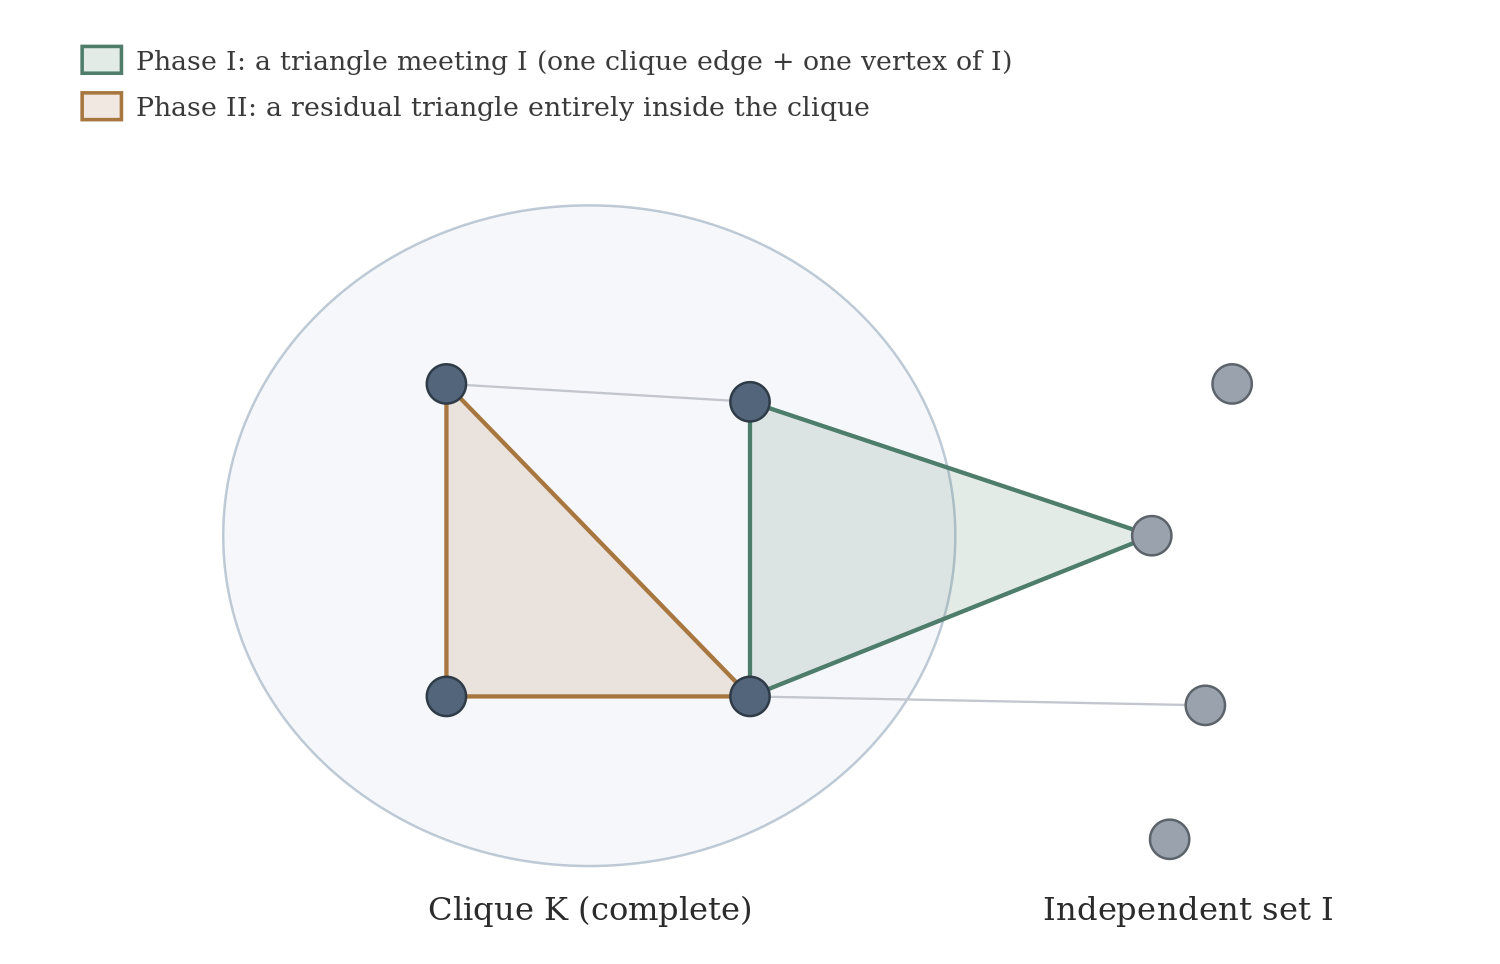
\includegraphics[keepaspectratio,alt={The two-phase fractional packing.}]{Figures/fig1_two_phase_packing_en.png}}
\caption{The two-phase fractional packing.}
\end{figure}

\textbf{Figure 1.} The two-phase fractional packing. Phase I packs triangles meeting the independent set (each uses one clique edge and one vertex of \(I\)); the residual capacity remaining on the clique edges then supports Phase II, a packing by triangles lying entirely inside the clique.

\subsubsection{4.1 Phase I}\label{phase-i}

For each clique edge \(e\), define

\[
\lambda_e
:=
\begin{cases}
1,&\kappa_e=0,\\[1mm]
\min\{1,\kappa_e^{-1}\},&\kappa_e>0.
\end{cases}
\]

For every triangle \(vxy\) with \(v\in I_{\ge2}\) and \(x,y\in N(v)\), assign

\[
w_1(vxy)
:=
\frac{\lambda_{xy}}{d_v-1}.
\tag{4.1}
\]

The load on a clique edge \(e\) is

\[
\lambda_e\kappa_e
=
\min\{\kappa_e,1\}.
\tag{4.2}
\]

A cross edge \(vx\) lies in at most \(d_v-1\) such triangles, each of weight at most \(1/(d_v-1)\). Thus \(w_1\) is feasible.

Define

\[
H:=\{e:\kappa_e\ge1\},
\qquad
L:=\{e:\kappa_e<1\}.
\]

Every positive Phase-I triangle contains exactly one clique edge. Hence

\[
|w_1|
=
|H|+\sum_{e\in L}\kappa_e.
\tag{4.3}
\]

\subsubsection{4.2 Phase II}\label{phase-ii}

The residual capacity on a clique edge is

\[
r_e:=\max\{1-\kappa_e,0\}.
\tag{4.4}
\]

Let \(w_2\) be an optimal fractional packing of clique triangles under these residual capacities. The finite packing-covering duality used here is recorded explicitly in Appendix B.

After capping the dual cover variables at one, substitute

\[
y_e:=1-x_e.
\]

The triangle-cover constraints become

\[
\sum_{e\in E(T)}y_e\le2.
\]

The coefficients \(1-\kappa_e\) are nonpositive on \(H\), so the maximizing vector may be taken to vanish there. A second substitution,

\[
z_e:=1-y_e,
\]

gives \(z_e=x_e\) and leads to the fixed capped-dual polytope

\[
\mathcal P_p
:=
\left\{
z\in[0,1]^{E(K)}:
\sum_{e\in E(T)}z_e\ge1
\text{ for every triangle }T\subseteq K
\right\}.
\tag{4.5}
\]

Define

\[
M(\kappa)
:=
\min_{z\in\mathcal P_p}
\sum_{e\in E(K)}(1-\kappa_e)z_e.
\tag{4.6}
\]

Let

\[
w_{\mathrm{com}}:=w_1+w_2,
\qquad
V_{\mathrm{com}}:=|w_{\mathrm{com}}|.
\]

Here \(M(\kappa)\) is the value of a residual cover problem, not the value of an additional packing. Its feasible region depends only on the clique size \(p\), while all information from the independent-set neighborhoods enters through the objective coefficients \(1-\kappa_e\).

The contribution of the edges in \(H\) can be accounted for explicitly. Lemma 3.1 and (4.3) give

\[
|w_1|
=
\frac{b_{\ge2}}2+\sum_{e\in H}(1-\kappa_e).
\]

On \(H\), the residual coefficient \(r_e\) is zero. In (4.6), by contrast, \(1-\kappa_e\le0\); since increasing \(z_e\) preserves feasibility, a minimizer may be chosen with \(z_e=1\) on every edge of \(H\). Thus the \(H\)-part of \(M(\kappa)\) is exactly \(\sum_{e\in H}(1-\kappa_e)\), while its restriction to \(L\) is the residual dual value \(|w_2|\). Equivalently,

\[
|w_2|=M(\kappa)-\sum_{e\in H}(1-\kappa_e).
\]

Adding the two displayed identities gives

\[
\boxed{
V_{\mathrm{com}}
=
\frac{b_{\ge2}}2+M(\kappa).
}
\tag{4.7}
\]

The packing is feasible: on a clique edge, the Phase-I and residual loads add to at most

\[
\min\{\kappa_e,1\}
+
\max\{1-\kappa_e,0\}
=
1.
\]

Therefore

\[
V_{\mathrm{com}}\le\nu_3^*(G).
\tag{4.8}
\]

Combining (2.1) and (4.7) yields

\[
\boxed{
|E(G)|-2V_{\mathrm{com}}
=
\binom{p}{2}-2M(\kappa)+b_1.
}
\tag{4.9}
\]

This cancellation is the bridge from the packing construction to the profile problem.

\begin{center}\rule{0.5\linewidth}{0.5pt}\end{center}

\subsection{5. Affine reduction to a pure neighborhood}\label{affine-reduction-to-a-pure-neighborhood}

For every set \(S\subseteq K\) with \(|S|\ge2\), define

\[
a_e^S
:=
\frac{\mathbf1_{\{e\subseteq S\}}}{|S|-1}.
\tag{5.1}
\]

Let \(n_S\) be the number of vertices \(v\in I_{\ge2}\) with \(N(v)=S\). Then

\[
\kappa=\sum_Sn_Sa^S.
\tag{5.2}
\]

Assume first that \(q>0\), and set

\[
\lambda_S:=\frac{n_S}{q},
\qquad
\kappa^S:=qa^S.
\]

Then

\[
\kappa=\sum_S\lambda_S\kappa^S,
\qquad
\lambda_S\ge0,
\qquad
\sum_S\lambda_S=1.
\tag{5.3}
\]

The reduction follows from an elementary concavity fact.

\paragraph{Lemma 5.1}\label{lemma-5.1}

Let \(P\) be nonempty and define the value function

\[
m(c):=\min_{x\in P}\langle c,x\rangle.
\]

If \(c=\sum_i\lambda_ic^{(i)}\) is a convex combination, then

\[
m(c)
\ge
\sum_i\lambda_i m(c^{(i)})
\ge
\min_i m(c^{(i)}).
\]

\paragraph{Proof}\label{proof-1}

For every \(x\in P\),

\[
\langle c,x\rangle
=
\sum_i\lambda_i\langle c^{(i)},x\rangle
\ge
\sum_i\lambda_i m(c^{(i)}).
\]

Take the minimum over \(x\in P\).

The residual value from Section 4.2 satisfies \(M(\kappa)=m(1-\kappa)\) when the generic polytope is \(P=\mathcal P_p\); the different letters distinguish the generic concavity lemma from the manuscript-specific residual notation.

Apply the lemma to the objective vectors \(1-\kappa^S\) over the fixed polytope \(\mathcal P_p\). The conclusion is a lower-bound reduction: a mixed profile need not coincide with any pure profile, but its residual value is at least the corresponding average of the pure-profile values. We obtain

\[
\boxed{
M(\kappa)
\ge
\sum_S\lambda_SM(\kappa^S)
\ge
\min_SM(\kappa^S).
}
\tag{5.4}
\]

It remains to control a pure profile.

\begin{center}\rule{0.5\linewidth}{0.5pt}\end{center}

\paragraph{Remark (fixed-polytope concavity)}\label{remark-fixed-polytope-concavity}

The reduction just used is an instance of a purely convex-analytic fact, stated here in abstract form. Fix a feasible polytope that does not depend on the profile and an objective that depends affinely on the profile mass \(\mu=(\mu_S)\). Because the optimal value of a linear program over a fixed polytope is concave in its objective vector, the value at a mixed profile dominates the corresponding convex combination of pure-profile values, and hence their minimum:
\[
M_b(\kappa_\mu)\ \ge\ \sum_S \tfrac{\mu_S}{q}\,M_b(\kappa^{S,q})\ \ge\ \min_S M_b(\kappa^{S,q}).
\]
This is recorded in the formal development as \texttt{lpVal\_concave} and \texttt{lpVal\_ge\_min}. A companion estimate, \texttt{lpVal\_lipschitz}, bounds the change in the fractional value when the baseline or the profile distribution is perturbed. It is intended for robust and near-split variants. Both are stated for a fixed feasible polytope with an affinely varying objective; neither requires symmetry, which enters only afterwards, on a single pure profile, in Section 6.

\subsection{6. The pure-profile orbit program}\label{the-pure-profile-orbit-program}

\begin{figure}
\centering
\pandocbounded{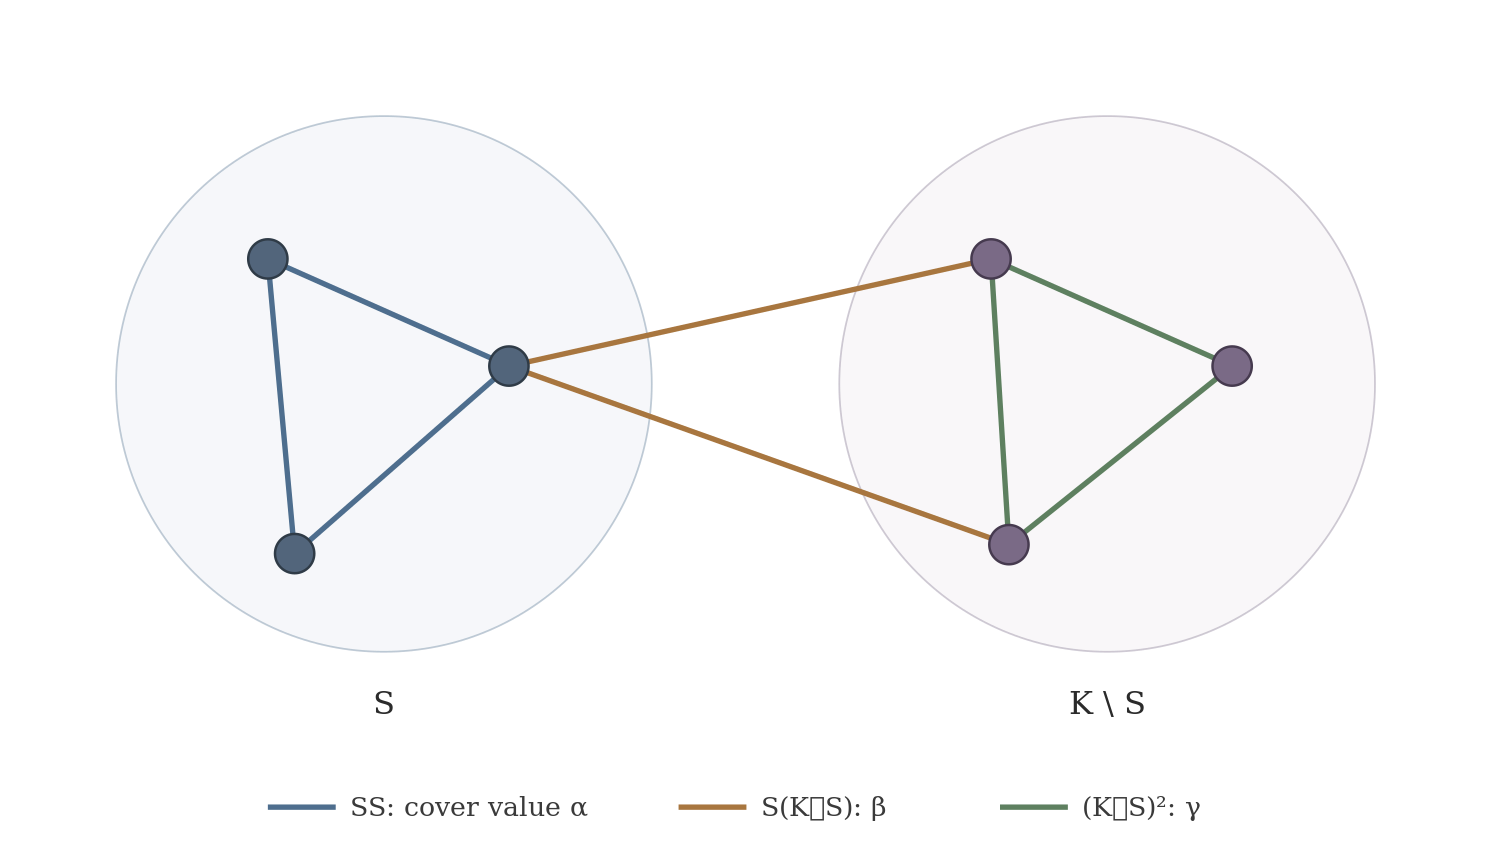
\includegraphics[keepaspectratio,alt={The three edge orbits of a pure profile.}]{Figures/fig2_three_orbits_en.png}}
\caption{The three edge orbits of a pure profile.}
\end{figure}

\textbf{Figure 2.} For a pure profile \(S\subseteq K\), the clique edges split into three orbits --- \(SS\), \(S(K\setminus S)\), and \((K\setminus S)(K\setminus S)\) --- on which the averaged cover is constant, with values \(\alpha,\beta,\gamma\) respectively.

Fix \(S\subseteq K\), and write

\[
s:=|S|,
\qquad
o:=p-s.
\]

For the pure profile,

\[
\kappa_e^S
=
\begin{cases}
q/(s-1),&e\subseteq S,\\
0,&\text{otherwise}.
\end{cases}
\tag{6.1}
\]

Average an optimal cover over the stabilizer of \(S\). Both the cover polytope and the pure-profile objective are invariant under this group. Averaging therefore preserves feasibility and objective value. The averaged cover is constant on the three edge orbits:

\[
SS,\qquad
S(K\setminus S),\qquad
(K\setminus S)(K\setminus S).
\]

Call the corresponding values

\[
\alpha,\qquad\beta,\qquad\gamma.
\]

The objective is

\[
A\alpha+B\beta+C\gamma,
\tag{6.2}
\]

where

\[
A:=\frac{s(s-1-q)}2,
\qquad
B:=so,
\qquad
C:=\frac{o(o-1)}2.
\tag{6.3}
\]

The existing triangle types impose

\[
3\alpha\ge1,
\qquad
\alpha+2\beta\ge1,
\qquad
2\beta+\gamma\ge1,
\qquad
3\gamma\ge1,
\tag{6.4}
\]

with any constraint omitted when its triangle type does not exist.

The feasible region is now a three-dimensional polytope. Its relevant extreme points give the uniform, separated, and hot-set covers; when some triangle types do not exist, the corresponding boundary regimes must be treated separately. Solving this three-variable program gives

\[
M(\kappa^S)
=
\begin{cases}
\min\{U,D\},&o\le2,\\[1mm]
\min\{U,D,H\},&o\ge3,
\end{cases}
\tag{6.5}
\]

where

\[
U:=\frac{A+B+C}{3},
\qquad
D:=A+C,
\qquad
H:=A+\frac{B+C}{3}.
\tag{6.6}
\]

The three values correspond to the uniform cover, the separated cover, and the hot-set cover.

\textbf{Table 1. The three-orbit cover program.} For a pure profile \(S\subseteq K\) with \(s=|S|\), \(o=p-s\), the residual objective is \(A\alpha+B\beta+C\gamma\) over the edge orbits \(SS\), \(S(K\setminus S)\), \((K\setminus S)(K\setminus S)\), and its minimum is attained at one of three named covers.

{\def\LTcaptype{none} % do not increment counter
\begin{longtable}[]{@{}lll@{}}
\toprule\noalign{}
Cover & Value & Orbit values \((\alpha,\beta,\gamma)\) \\
\midrule\noalign{}
\endhead
\bottomrule\noalign{}
\endlastfoot
Uniform \(U\) & \((A+B+C)/3\) & \((\tfrac13,\tfrac13,\tfrac13)\) \\
Separated \(D\) & \(A+C\) & \((1,0,1)\) \\
Hot-set \(H\) & \(A+(B+C)/3\) & \((1,\tfrac13,\tfrac13)\) \\
\end{longtable}
}

with \(A=\tfrac{s(s-1-q)}2\), \(B=so\), \(C=\tfrac{o(o-1)}2\); and \(M(\kappa^S)=\min\{U,D\}\) for \(o\le2\), \(\min\{U,D,H\}\) for \(o\ge3\) (Appendix A).

\begin{center}\rule{0.5\linewidth}{0.5pt}\end{center}

\subsection{7. A uniform lower bound for the residual cover}\label{a-uniform-lower-bound-for-the-residual-cover}

Define

\[
R(p,q)
:=
\frac{2p^2-2pq-q^2}{12}.
\tag{7.1}
\]

We compare each candidate in (6.5) with \(R(p,q)\).

For the uniform candidate, using \(o=p-s\),

\[
12(U-R)
=
q(2o+q)-2p.
\tag{7.2}
\]

Since \(q,o\ge0\),

\[
U-R\ge-\frac p6.
\tag{7.3}
\]

For the separated candidate,

\[
12(D-R)
=
12o^2-6o(2p-q)+(2p-q)^2-6p.
\tag{7.4}
\]

The quadratic part is nonnegative because

\[
12u^2-6uv+v^2
=
12\left(u-\frac v4\right)^2+\frac{v^2}{4}.
\]

Thus

\[
D-R\ge-\frac p2.
\tag{7.5}
\]

For the hot-set candidate,

\[
12(H-R)
=
(2s-q)^2+2q(p-s)-2p-4s.
\tag{7.6}
\]

The first two terms are nonnegative, and \(s\le p\), so

\[
H-R\ge-\frac p2.
\tag{7.7}
\]

Consequently,

\[
M(\kappa^S)
\ge
R(p,q)-\frac p2
\]

for every pure profile. By (5.4),

\[
\boxed{
M(\kappa)
\ge
R(p,q)-\frac p2.
}
\tag{7.8}
\]

When \(q=0\), the same estimate follows directly. If \(p\le2\), then \(M(0)=0\). If \(p\ge3\), the constant cover \(z_e=1/3\) is feasible. To see that it is optimal, sum the cover constraints over all clique triangles: every clique edge occurs in exactly \(p-2\) such triangles, which gives the matching lower bound. Hence

\[
M(0)=\frac{p(p-1)}6.
\]

\begin{center}\rule{0.5\linewidth}{0.5pt}\end{center}

\paragraph{Remark (where the estimate is tight)}\label{remark-where-the-estimate-is-tight}

The three comparisons above are far from tight except at one configuration. Writing \(o=p-s\), the slack \(M(\kappa^S)-\big(R(p,q)-p/2\big)\) is at least \(9/4\) whenever \(s\ge3\) and \(o\ge3\), and at least \(1/4\) in each of the regimes \(s=2\) with \(o\ge1\), \(o=1\), and \(o=2\). Equality occurs only for \(o=0\) together with \(q=2p\): the pure profile whose neighborhood is the whole clique in a graph with \(|I|=2|K|\), which is exactly the complete-split extremizer \(K_p\vee\overline K_{2p}\) evaluated in Section 9 and identified by Paper II as the terminal family of the fractional extremal problem. Thus the point \((p,q,s)=(2,4,2)\) on the \(s=2\) boundary belongs to the equality family; away from \(o=0\), the \(s=2\) boundary has slack at least \(1/4\). Appendix A treats the boundary regimes in full because the minimum of the orbit program genuinely changes form there.

\subsection{8. Proof of the main theorem}\label{proof-of-the-main-theorem}

Start from (4.9):

\[
|E(G)|-2V_{\mathrm{com}}
=
\binom p2-2M(\kappa)+b_1.
\]

Insert (7.8):

\[
|E(G)|-2V_{\mathrm{com}}
\le
\binom p2-2R(p,q)+p+b_1.
\tag{8.1}
\]

A direct simplification gives

\[
\binom p2-2R(p,q)+p
=
\frac{(p+q)^2}{6}+\frac p2.
\tag{8.2}
\]

Hence

\[
|E(G)|-2V_{\mathrm{com}}
\le
\frac{(p+q)^2}{6}+\frac p2+b_1.
\tag{8.3}
\]

Write \(n=p+q+b_1+|I_0|\) from (2.2), where \(I_0\) is the set of isolated independent vertices. Rather than bounding the quadratic and linear terms of (8.3) separately, subtract (8.3) from the target with sharp quadratic coefficient:

\[
\frac{n^2}{6}+\frac n2-\Big[\frac{(p+q)^2}{6}+\frac p2+b_1\Big]
=
\frac{b_1^2+|I_0|^2+2b_1|I_0|+2(b_1+|I_0|)(p+q)+3|I_0|+3q-3b_1}{6}.
\]

Every term on the right is nonnegative except \(-3b_1\). If \(b_1=0\) the inequality is immediate. If \(b_1\ge1\), then \(p\ge1\), because a degree-one independent vertex has its neighbor in \(K\); grouping \(2b_1(p+q)-3b_1=b_1(2p+2q-3)\) shows this is nonnegative whenever \(p+q\ge2\). The residual regime is \(p=1,\ q=0\), where the difference reduces to

\[
\frac{b_1(b_1-1)+|I_0|^2+2b_1|I_0|+5|I_0|}{6}\ge0,
\]

with equality exactly when \(b_1=1\) and \(|I_0|=0\). Hence

\[
|E(G)|-2V_{\mathrm{com}}
\le
\frac{n^2}{6}+\frac n2.
\tag{8.4}
\]

Finally, \(V_{\mathrm{com}}\le\nu_3^*(G)\). Thus

\[
|E(G)|-2\nu_3^*(G)
\le
|E(G)|-2V_{\mathrm{com}}
\le
\frac{n^2}{6}+\frac n2.
\]

This proves Theorem 1.1.

\begin{center}\rule{0.5\linewidth}{0.5pt}\end{center}

\subsection{9. Discussion}\label{discussion}

Three elementary ideas drive the proof. We first separate the packing into a part supported on triangles meeting the independent set and a residual part supported entirely on the clique. We then formulate the residual problem over one fixed cover polytope. Symmetry is used only after the lower-bound problem has been reduced to pure profiles.

The fixed-polytope feature is the central structural point. Concavity applies because the feasible region does not change when the neighborhood profile changes; only the objective vector does. If the constraints themselves depended on the profile, the reduction in Section 5 would no longer follow from the same argument. Orbit averaging is a separate step: it uses the symmetry of a pure profile and is not needed for the affine reduction itself.

The intermediate quantities \(p\), \(q\), and \(\kappa\) depend on the chosen split presentation. The final estimate does not. Once the terms are assembled, the conclusion is expressed only in terms of \(n=|V(G)|\).

The additive term \(n/2\) in Theorem 1.1 is not optimized. For the complete-split family \(K_p\vee\overline{K}_{2p}\), with \(p\ge2\) and \(n=3p\), every triangle uses at least one clique edge, so \(\nu_3^*(G)\le\binom p2\), while the Phase-I construction attains equality. Consequently, the left-hand side of Theorem 1.1 equals \(n^2/6+n/6\) on this family, so the optimal additive term lies between \(n/6\) and the \(n/2\) proved here. Determining it exactly is outside the scope of the present argument.

The paper is intentionally limited to the finite fractional inequality. Any passage to integral triangle packings, clique partitions, asymptotic consequences, or wider graph classes requires additional results and belongs to a separate stage.

The reusable component is the fixed-polytope affine reduction, which is independent of the particular finite bound proved here.

Paper III of the series later reuses the same pure-profile three-orbit computation in an integral setting. With its notation \(d=s\) and \(p-d=o\), the three branches of its common-profile value \(F(p,q,d)\) are \(qd/2+U\), \(qd/2+D\), and \(qd/2+H\), where \(qd/2\) is the Phase-I contribution of the pure profile in the present paper; its term \(C_\alpha p^2\), for \(\alpha=q/p\), is the comparison value \(R(p,q)\) of Section 7. This is a forward cross-reference only: no result of Paper III is used here.

\begin{center}\rule{0.5\linewidth}{0.5pt}\end{center}

\subsection{10. Reproducibility and proof record}\label{reproducibility-and-proof-record}

The proof is analytic. Computational experiments were used during development to search for counterexamples and detect transcription errors, but no computation is a logical premise of the theorem. For that reason, computational regression material is kept outside the paper rather than included as a second appendix.

The accompanying calculation ledger records:

\begin{itemize}
\tightlist
\item
  every exact identity;
\item
  every inequality direction;
\item
  the complete loss accounting;
\item
  the branch \(q=0\);
\item
  the orbit regimes;
\item
  the final conversion to \(n\).
\end{itemize}

The author reports an internal AI-assisted adversarial audit of the theorem statement, quantitative bound, and proof assembly. This is a validation record, not a claim of external peer review.

\subsubsection{Formalization status in Lean}\label{formalization-status-in-lean}

The snapshot at \texttt{PAPER\_I/05\_formalization/lean\_v1.2\_freeze} contains the Lean sources and a successful recorded 8,034-job build against Lean 4 / Mathlib v4.28.0 {[}6,7{]}. It contains \texttt{paperI\_main\_sharp}, whose statement is \texttt{Phi\ ≤\ n\^{}2/6\ +\ n/2}, together with the weaker companion declaration \texttt{paperI\_main} and the interface results listed below. Its axiom gate also queries \texttt{PaperI.assembly\_sharp} and \texttt{PaperI.Split.residual\_duality}. Appendix C records the main declaration. The exact archive was subsequently reproduced in an external clean room with the same 8,034-job result and the same theorem-level axiom footprint.

The frozen axiom report records only Lean's standard foundational axioms, \texttt{propext}, \texttt{Classical.choice}, and \texttt{Quot.sound}, for the main theorem and the listed declarations; it records no project-level mathematical axiom. These are logical foundations used throughout Mathlib, not additional mathematical assumptions of the paper.

The release artifact also records the finite-dimensional packing-covering duality used in Proposition B.1. In Lean it appears as \texttt{residual\_duality}, an application of the general theorem \texttt{covering\_packing\_duality}. The artifact records that theorem as derived from a finite Farkas lemma and Mathlib's closed-cone infrastructure, rather than postulated as an external axiom. Schrijver {[}4, Chapter 7{]} remains the classical reference for the written proof.

The frozen source archive is \texttt{PAPER\_I\_lean\_v1.2\_freeze.zip}, with SHA-256 \texttt{0181506408644fc1f8872d711de5a98a500f4052aa295bcd6f8c82776694fd3a}. It is stored under \texttt{PAPER\_I/05\_formalization/lean\_v1.2\_freeze} and excludes project caches and compiled objects. The freeze build target includes several \texttt{Contrib} modules used for possible upstreaming; that contribution lane is a byproduct and is not part of the paper's trusted mathematical assumptions. The axiom report above controls the logical dependency statement. The external clean-room reproduction applies to these exact archive bytes; the manuscript revision does not alter the formal artifact.

\begin{center}\rule{0.5\linewidth}{0.5pt}\end{center}

\subsection{Appendix A. The three-orbit program and its boundary cases}\label{appendix-a.-the-three-orbit-program-and-its-boundary-cases}

This appendix supplies the details behind (6.5). It is included because the cases in which one of the four triangle types does not exist are easy to obscure in a compressed orbit calculation.

For a pure profile \(S\subseteq K\), write

\[
s:=|S|,
\qquad
o:=p-s,
\]

and let \(\alpha,\beta,\gamma\) denote the cover values on the edge orbits

\[
SS,\qquad S(K\setminus S),\qquad (K\setminus S)(K\setminus S).
\]

The objective is

\[
A\alpha+B\beta+C\gamma,
\]

where

\[
A=\frac{s(s-1-q)}2,
\qquad
B=so,
\qquad
C=\frac{o(o-1)}2.
\]

Only constraints corresponding to existing triangle types are imposed.

\subsubsection{\texorpdfstring{A.1 The interior case \(s\ge3\) and \(o\ge3\)}{A.1 The interior case s\textbackslash ge3 and o\textbackslash ge3}}\label{a.1-the-interior-case-sge3-and-oge3}

All four constraints are present:

\[
3\alpha\ge1,
\qquad
\alpha+2\beta\ge1,
\qquad
2\beta+\gamma\ge1,
\qquad
3\gamma\ge1.
\]

If \(A<0\), decreasing the objective favors the largest feasible value of \(\alpha\), so an optimum has \(\alpha=1\). The remaining lower boundary joins

\[
(\beta,\gamma)=(0,1)
\]

and

\[
(\beta,\gamma)=\left(\frac13,\frac13\right).
\]

Because the objective is linear on that segment, its minimum is attained at an endpoint. These two endpoint values are

\[
D=A+C
\]

and

\[
H=A+\frac{B+C}{3}.
\]

If \(A\ge0\), then for fixed \(\beta\) the least feasible values of \(\alpha\) and \(\gamma\) are

\[
\alpha=\gamma=\max\left\{\frac13,1-2\beta\right\}.
\]

For \(0\le\beta\le1/3\), the objective is linear between the separated point and the uniform point, with values \(D\) and

\[
U=\frac{A+B+C}{3}.
\]

For \(\beta\ge1/3\), the objective is

\[
U+B\left(\beta-\frac13\right)\ge U,
\]

because \(B\ge0\). Hence the minimum is one of \(U,D,H\).

\subsubsection{\texorpdfstring{A.2 The case \(s=2\)}{A.2 The case s=2}}\label{a.2-the-case-s2}

The \(SSS\) triangle type does not exist, so the constraint \(3\alpha\ge1\) is omitted.

If \(A<0\), the same monotonicity argument gives \(\alpha=1\), and the endpoint analysis above remains valid.

If \(A\ge0\) and \(o\ge3\), the missing constraint introduces one additional boundary endpoint at \(\beta=1/2\). Its objective value exceeds the uniform value by

\[
\frac{B-2A}{6}.
\]

For \(s=2\),

\[
B-2A
=
2o-2(1-q)
=
2(o+q-1)\ge0
\]

whenever this endpoint is relevant. Therefore it does not improve on \(U\). The cases \(o=0,1,2\), in which some triangle types and their constraints are absent, are treated separately in A.3; the excess formula above is not invoked there.

\subsubsection{\texorpdfstring{A.3 The cases \(o=0,1,2\)}{A.3 The cases o=0,1,2}}\label{a.3-the-cases-o012}

When \(o=0\), we have \(B=C=0\). If \(s\ge3\), the only triangle constraint is \(3\alpha\ge1\), so

\[
\min_{\alpha\in[1/3,1]}A\alpha
=
\min\left\{\frac A3,A\right\}
=
\min\{U,D\}.
\]

If \(s=2\), then \(p=2\) and there are no clique-triangle constraints. Since the pure-profile case has \(q>0\), we have \(A=1-q\le0\), and the minimum over \(0\le\alpha\le1\) is \(A=D\). Thus the formula \(\min\{U,D\}\) remains valid.

When \(o=1\), there are no \((K\setminus S)^2\) edges and no triangle type entirely in \(K\setminus S\). The reduced feasible region is an interval, and its endpoints give \(U\) or \(D\).

When \(o=2\), the triangle type entirely in \(K\setminus S\) does not exist. A possible extra endpoint has

\[
(\beta,\gamma)=\left(\frac12,0\right)
\]

and objective value

\[
A+\frac B2.
\]

Since \(o=2\),

\[
\frac B2=s
\qquad\text{and}\qquad
C=1,
\]

so

\[
A+\frac B2\ge A+C=D.
\]

Thus this endpoint is dominated by \(D\).

Consequently,

\[
M(\kappa^S)
=
\begin{cases}
\min\{U,D\},&o\le2,\\[1mm]
\min\{U,D,H\},&o\ge3.
\end{cases}
\]

No nonexistent orbit or triangle constraint is used in any boundary regime.

\begin{center}\rule{0.5\linewidth}{0.5pt}\end{center}

\subsection{Appendix B. Finite packing-covering duality}\label{appendix-b.-finite-packing-covering-duality}

For completeness, we record the specialized finite packing-covering dual pair used in Section 4, prove weak duality, verify the hypotheses required for the finite-dimensional strong linear-programming duality theorem cited below, and apply that theorem to the residual program.

\paragraph{Proposition B.1}\label{proposition-b.1}

Let \(\mathcal T\) be a finite family of triangles, let \(E\) be the finite set of edges appearing in them, and let \(r=(r_e)_{e\in E}\) be a nonnegative capacity vector. Then

\[
\max\left\{
\sum_{T\in\mathcal T}w_T:
w_T\ge0,\ 
\sum_{T\ni e}w_T\le r_e
\text{ for every }e\in E
\right\}
\]

equals

\[
\min\left\{
\sum_{e\in E}r_ex_e:
x_e\ge0,\ 
\sum_{e\in E(T)}x_e\ge1
\text{ for every }T\in\mathcal T
\right\}.
\]

Both optima are attained.

\paragraph{Proof}\label{proof-2}

Let \(A\) be the edge-triangle incidence matrix, so that \(A_{eT}=1\) when \(e\in E(T)\) and \(A_{eT}=0\) otherwise. The two programs are

\[
\max\{\mathbf 1^{\mathsf T}w:Aw\le r,\ w\ge0\}
\]

and

\[
\min\{r^{\mathsf T}x:A^{\mathsf T}x\ge\mathbf 1,\ x\ge0\}.
\]

Weak duality follows directly. Indeed, for every feasible pair \(w,x\),

\[
\mathbf 1^{\mathsf T}w
\le
x^{\mathsf T}Aw
\le
x^{\mathsf T}r.
\]

The primal feasible region is nonempty, since \(w=0\) is feasible. It is also bounded in every coordinate: if \(T\in\mathcal T\), then for each edge \(e\in E(T)\),

\[
0\le w_T\le\sum_{T'\ni e}w_{T'}\le r_e.
\]

Hence the primal optimum is finite and attained. The dual is feasible, for example with \(x_e=1\) for every \(e\). Finite-dimensional strong linear-programming duality {[}4, Chapter 7{]} therefore gives equality of the two attained optimum values. Applying the proposition to the clique triangles and the residual capacities \(r_e\) in (4.4) yields the dual program used in Section 4.

\textbf{Formalization note.} The v1.2 freeze records Proposition B.1 as the Lean declaration \texttt{PaperI.Split.residual\_duality}, an instance of the general finite strong-duality theorem \texttt{covering\_packing\_duality}. The artifact records the latter as proved from a finite Farkas lemma, using the closedness of a finitely generated convex cone and the hyperplane-separation theorem for closed convex cones. Thus the duality used here is derived inside the formal development, not postulated as a project-specific axiom. Schrijver remains the classical reference for the written argument. The corresponding sources, build log, and axiom report are delivered in \texttt{PAPER\_I/05\_formalization/lean\_v1.2\_freeze}.

\begin{center}\rule{0.5\linewidth}{0.5pt}\end{center}

\subsection{Appendix C. Formalized statement}\label{appendix-c.-formalized-statement}

The accompanying formal artifact records the following Lean 4 declaration for Theorem 1.1:

\begin{Shaded}
\begin{Highlighting}[]
\NormalTok{theorem paperI\_main\_sharp (G : Split) :}
\NormalTok{    G.Phi ≤ (G.n : \ensuremath{\mathbb{R}}) \^{} 2 / 6 + (G.n : \ensuremath{\mathbb{R}}) / 2}

\NormalTok{{-}{-} weaker companion form (larger additive term):}
\NormalTok{theorem paperI\_main (G : Split) :}
\NormalTok{    G.Phi ≤ (G.n : \ensuremath{\mathbb{R}}) \^{} 2 / 6 + (G.n : \ensuremath{\mathbb{R}})}
\end{Highlighting}
\end{Shaded}

Here \texttt{Split} packages the data of a split graph used in the proof: a clique of size \texttt{p}, an independent vertex type, and the neighborhoods of the independent vertices inside the clique. The field \texttt{n} is the total number of vertices. The quantity \texttt{Phi} is defined as \texttt{\textbar{}E\textbar{}\ −\ 2·nu3star}, where \texttt{nu3star} is the supremum of the feasible fractional triangle-packing values. Elsewhere in the series this fractional deficit is written \(\Phi^*\), while the unstarred \(\Phi\) is reserved for the integral deficit \(|E(G)|-2\nu_3(G)\); the Lean identifier is retained to match the recorded declaration. With these definitions, \texttt{paperI\_main\_sharp} is precisely

\[
|E(G)|-2\nu_3^*(G)\le \frac{n^2}{6}+\frac{n}{2},
\]

the inequality stated in Theorem 1.1 (declaration \texttt{paperI\_main\_sharp}). The companion declaration \texttt{paperI\_main} records the weaker additive term \(n\).

The supplied build report records zero \texttt{sorry}. The supplied axiom report is:

\begin{Shaded}
\begin{Highlighting}[]
\NormalTok{PaperI.Split.paperI\_main\_sharp depends on axioms: [propext, Classical.choice, Quot.sound]}
\NormalTok{PaperI.paperI\_main         depends on axioms: [propext, Classical.choice, Quot.sound]}
\NormalTok{PaperI.assembly\_sharp      depends on axioms: [propext, Classical.choice, Quot.sound]}
\NormalTok{PaperI.Split.residual\_duality depends on axioms: [propext, Classical.choice, Quot.sound]}
\end{Highlighting}
\end{Shaded}

These are the three standard foundational axioms of Lean and Mathlib. No project-specific axiom is used.

\textbf{Table 2. Frozen formalization perimeter (Lean v1.2 freeze).} The frozen Lean 4 / Mathlib v4.28.0 snapshot records the proved core with only Lean's standard foundational axioms and no project-level mathematical axiom. An external clean-room build and theorem-level axiom check reproduced the exact archive.

{\def\LTcaptype{none} % do not increment counter
\begin{longtable}[]{@{}
  >{\raggedright\arraybackslash}p{(\linewidth - 4\tabcolsep) * \real{0.3333}}
  >{\raggedright\arraybackslash}p{(\linewidth - 4\tabcolsep) * \real{0.3333}}
  >{\raggedright\arraybackslash}p{(\linewidth - 4\tabcolsep) * \real{0.3333}}@{}}
\toprule\noalign{}
\begin{minipage}[b]{\linewidth}\raggedright
Node
\end{minipage} & \begin{minipage}[b]{\linewidth}\raggedright
Statement
\end{minipage} & \begin{minipage}[b]{\linewidth}\raggedright
Axiom footprint
\end{minipage} \\
\midrule\noalign{}
\endhead
\bottomrule\noalign{}
\endlastfoot
\texttt{paperI\_main\_sharp} (Theorem 1.1) & \(\lvert E(G)\rvert-2\nu_3^*(G)\le n^2/6+n/2\) & \texttt{propext}, \texttt{Classical.choice}, \texttt{Quot.sound} \\
\texttt{paperI\_main} (weaker companion bound) & \(\lvert E(G)\rvert-2\nu_3^*(G)\le n^2/6+n\) & \texttt{propext}, \texttt{Classical.choice}, \texttt{Quot.sound} \\
\texttt{lpVal\_concave}, \texttt{lpVal\_ge\_min} (§5 interface) & abstract concavity / pure-profile lower bound & \texttt{propext}, \texttt{Classical.choice}, \texttt{Quot.sound} \\
\texttt{lpVal\_lipschitz} (§5 interface) & parametric stability of the fractional value & \texttt{propext}, \texttt{Classical.choice}, \texttt{Quot.sound} \\
\texttt{residual\_duality} (Prop. B.1) & finite packing--covering duality & \texttt{propext}, \texttt{Classical.choice}, \texttt{Quot.sound} \\
\end{longtable}
}

\subsection{Acknowledgements}\label{acknowledgements}

The author is deeply grateful to his wife María Paz and to his children Lucas, Juan Cristóbal, Francisca, Raimundo, and Benjamín for their love, patience, and support.

\begin{center}\rule{0.5\linewidth}{0.5pt}\end{center}

\subsection{Use of AI-assisted tools}\label{use-of-ai-assisted-tools}

AI-assisted tools were used during exploratory, computational, adversarial, organizational, formalization-support, and editorial stages, including systems from Anthropic, Google, and OpenAI. They supported the testing of candidate arguments, exact regression checks, proof organization, audit preparation, and drafting. The author reviewed the mathematical content, selected the final arguments, and remains solely responsible for the claims, citations, code, and presentation. No AI system is listed as an author.

\begin{center}\rule{0.5\linewidth}{0.5pt}\end{center}

\subsection{References}\label{references}

{[}1{]} P. Erdős, E. T. Ordman, and Y. Zalcstein, ``Clique partitions of chordal graphs,'' \emph{Combinatorics, Probability and Computing} \textbf{2} (1993), no. 4, 409--415.

{[}2{]} G.-T. Chen, P. Erdős, and E. T. Ordman, ``Clique partitions of split graphs,'' in \emph{Combinatorics, Graph Theory, Algorithms and Applications} (Beijing, 1993), World Scientific, 1994, pp.~21--30, author-hosted scan: https://ordman.net/MathResearch/CEOClique\_Parts.pdf, accessed August 21, 2026.

{[}3{]} T. F. Bloom, ``Erdős Problem \#81,'' \emph{Erdős Problems}, https://www.erdosproblems.com/81, accessed August 21, 2026.

{[}4{]} A. Schrijver, \emph{Theory of Linear and Integer Programming}, Wiley-Interscience Series in Discrete Mathematics and Optimization, John Wiley \& Sons, Chichester, 1986.

{[}5{]} M. S. Cavers, \emph{Clique Partitions and Coverings of Graphs}, M.Math. essay, University of Waterloo, 2005.

{[}6{]} L. de Moura and S. Ullrich, ``The Lean 4 Theorem Prover and Programming Language,'' in \emph{Automated Deduction -- CADE 28}, Lecture Notes in Computer Science \textbf{12699}, Springer, 2021, pp.~625--635, https://doi.org/10.1007/978-3-030-79876-5\_37.

{[}7{]} The mathlib Community, ``The Lean Mathematical Library,'' in \emph{Proceedings of the 9th ACM SIGPLAN International Conference on Certified Programs and Proofs (CPP 2020)}, ACM, 2020, pp.~367--381, https://doi.org/10.1145/3372885.3373824.

\end{document}
